\section{Matrix Algebra}
\label{sect:matrix-algebra}
\begin{enumerate}
\item \emph{Linear algebra} is central to many areas of mathematics, and has
also many applications in fields outside mathematics, e.g., engineering,
economics, etc. It is related to \emph{linear equations} and \emph{linear
transformations} (between \emph{vector spaces}).

\item In linear algebra, a popular mathematical concept with wide applicability
is \emph{matrix}, which is essentially a rectangular array. So we will study it
in \cref{sect:matrix-algebra}. Nonetheless, from a mathematical point of view,
the more important (but also more abstract) concepts in linear algebra are
instead \emph{vector spaces} and \emph{linear transformations} (which are
somehow related to matrices, as we will see).

\item Before studying matrices, we shall illustrate the stricture and the
relationship between different topics in MATH2101:
\begin{center}
\begin{tikzpicture}
\node[draw] (ma) at (0,0) {Matrix algebra (\cref{sect:matrix-algebra})};
\node[draw, text width=3.5cm] (sle) at (-3,-2) {Systems of linear equations (\cref{sect:sle})};
\node[draw] (vs) at (4,-2) {Vector spaces (\cref{sect:vector-spaces})};
\node[draw, text width=4cm] (lt) at (3,-4) {Linear transformations (\cref{sect:linear-transformations})};
\node[draw] (ort) at (8,-4) {Orthogonalization (\cref{sect:orthogonalization})};
\node[draw] (diag) at (-1,-6) {Diagonalization (\cref{sect:diagonalization})};
\draw[-Latex] (ma) -- (sle)
node[midway,left]{application};
\draw[-Latex] (ma) -- (vs)
node[midway, right=0.3cm]{tools};
\draw[-Latex] (sle) -- (vs)
node[midway, above]{tools};
\draw[-Latex] (vs) -- (lt)
node[midway, left]{functions};
\draw[-Latex] (vs) -- (ort)
node[midway, right=0.3cm]{advanced topics};
\draw[-Latex] (ma) -- (diag)
node[midway, left]{advanced topics};
\end{tikzpicture}
\end{center}
\end{enumerate}
\subsection{Introduction to Matrices}
\begin{enumerate}
\item A \defn{matrix} is a rectangular array of objects (called
\defn{entries}). In MATH2101, each entry can be assumed to be a real number
(unless otherwise specified).

\begin{note}
Unless otherwise specified, we shall use capital letters (\(A\), \(B\), etc.)
to denote arbitrary matrices, and small letters \((s\), \(t\), etc.) to denote
arbitrary scalars (synonymous as real numbers in MATH2101).
\end{note}

\item Some terminologies:
\begin{itemize}
\item A horizontal (vertical) unit of a matrix is called a \defn{row}
(\defn{column}).
\begin{center}
\begin{tikzpicture}
\node[] () at (0,0) {\(\displaystyle \mqty[1&2&3&4\\ 1&4&5&8\\ 2&3&6&0]\)};
\draw[-Latex, blue] (-2,0.5) -- (-1.2,0.5)
node[pos=-1.5]{\(\displaystyle \mqty[1&2&3&4]\)};
\draw[-Latex, violet] (-2,0) -- (-1.2,0)
node[pos=-1.5]{\(\displaystyle \mqty[1&4&5&8]\)};
\draw[-Latex, orange] (-2,-0.5) -- (-1.2,-0.5)
node[pos=-1.5]{\(\displaystyle \mqty[2&3&6&0]\)};
\draw[very thick, decorate,decoration={mirror, calligraphic brace, amplitude=5pt, raise=0}] (-4.5,0.6) -- (-4.5,-0.6)
node[midway, left=0.2cm]{rows};
\end{tikzpicture}\\
\begin{tikzpicture}
\node[] () at (0,0) {\(\displaystyle \mqty[1&2&3&4\\ 1&4&5&8\\ 2&3&6&0]\)};
\draw[-Latex, blue] (-0.8,-1.5) -- (-0.8,-0.7)
node[pos=-1]{\(\displaystyle \mqty[1\\ 1\\ 2]\)};
\draw[-Latex, violet] (-0.25,-1.5) -- (-0.25,-0.7)
node[pos=-1]{\(\displaystyle \mqty[2\\ 4\\ 3]\)};
\draw[-Latex, orange] (0.3,-1.5) -- (0.3,-0.7)
node[pos=-1]{\(\displaystyle \mqty[3\\ 5\\ 6]\)};
\draw[-Latex, magenta] (0.8,-1.5) -- (0.8,-0.7)
node[pos=-1]{\(\displaystyle \mqty[4\\ 8\\ 0]\)};
\draw[very thick, decorate,decoration={mirror, calligraphic brace, amplitude=5pt, raise=0}] (-1,-3.2) -- (1,-3.2)
node[midway, below=0.2cm]{columns};
\end{tikzpicture}
\end{center}
\item A matrix with \(m\) rows and \(n\) columns is called an \defn{\(m\times
n\) matrix}, and we call \(m\times n\) the \defn{size} of the matrix.

\begin{note}
Each row (column) of an \(m\times n\) matrix can be viewed as a \(1\times n\)
(\(m\times 1\)) matrix.
\end{note}
\item The \defn{\((i,j)\)-entry} of a matrix is the entry in its \(i\)th row
and \(j\)th column. \begin{note}
Sometimes we denote the \((i,j)\)-entry of a matrix \(A\) by \(A_{ij}\).
\end{note}
\item A \defn{square matrix} is a matrix with the same number of rows and columns.
\item A \defn{submatrix} of a matrix \(M\) is a matrix whose rows and columns
are both subsets of those of \(M\), in the same relative order.
\item The \defn{main diagonal} of a matrix is the collection of all
\((i,j)\)-entries where \(i=j\).
\item A \defn{triangular matrix} is a square matrix that is either \emph{upper
triangular} or \emph{lower triangular}:
\begin{itemize}
\item A square matrix is \defn{upper triangular} if all entries below the \blc{main
diagonal} are \(0\). Example:
\[
\mqty[\blc{1}&2&3\\ \rc{0}&\blc{4}&5\\ \rc{0}&\rc{0}&\blc{6}]
\]
\item A square matrix is \defn{lower triangular} if all entries above the \blc{main
diagonal} are \(0\). Example:
\[
\mqty[\blc{1}&\rc{0}&\rc{0}\\2&\blc{3}&\rc{0}\\ 4&5&\blc{6}]
\]
\end{itemize}
\item A \defn{diagonal matrix} is a square matrix which is both upper and lower
triangular, i.e., its off-diagonal entries (entries not in the main diagonal)
are all \(0\).
Example:
\[
\mqty[1&\rc{0}&\rc{0}\\ \rc{0}&4&\rc{0}\\ \rc{0}&\rc{0}&6]
\]
\item Two matrices \(A\) and \(B\) are \defn{equal (\(A=B\))} if:
\begin{itemize}
\item they have the same size, and
\item their corresponding entries are equal, i.e., \(a_{ij}=b_{ij}\) for any
\(i\) and \(j\), where \(a_{ij}\) (\(b_{ij}\)) denote the \((i,j)\)-entry of
\(A\) (\(B\)).
\end{itemize}
\begin{note}
For convenience, sometimes we write \(A=[a_{ij}]\) to denote the
\((i,j)\)-entry of matrix \(A\) is \(a_{ij}\) (for any \(i\) and \(j\)). Also,
unless otherwise specified, \(a_{ij},b_{ij},c_{ij},\dotsc\) denote the
\((i,j)\) entry of matrices \(A,B,C,\dotsc\) respectively.
\end{note}
\end{itemize}
\end{enumerate}
\subsection{Operations on Matrices}
\label{subsect:matrix-operations}
\begin{enumerate}
\item \defn{Matrix addition} is defined \emph{entrywise}, i.e., if
\(A=[a_{ij}]\) and \(B=[b_{ij}]\), then
\[
A+B=[a_{ij}+b_{ij}].
\]
\begin{note}
Matrix addition is well-defined only when the two matrices involved have the
same size.
\end{note}
Examples:
\[
\mqty[\vc{1}&\vc{2}&\vc{3}\\ \vc{2}&\vc{3}&\vc{4}]
+\mqty[\blc{5}&\blc{1}&\blc{0}\\ \blc{2}&\blc{1}&\blc{4}]
=
\mqty[\vc{1}+\blc{5}&\vc{2}+\blc{1}&\vc{3}+\blc{0}\\ \vc{2}+\blc{2}&\vc{3}+\blc{1}&\vc{4}+\blc{4}],
\]
and
\[
\mqty[\vc{1}&\vc{2}&\vc{3}\\ \vc{2}&\vc{3}&\vc{4}]
+\mqty[\blc{5}&\blc{1}\\ \blc{2}&\blc{1}]
\text{ is not well-defined!}
\]
\item \label{it:matrix-add-asso-comm}
Matrix addition is both: 
\begin{enumerate}
\item \emph{commutative}, i.e., \(A+B=B+A\) for any matrices \(A\) and \(B\) of
the same size, and
\item \emph{associative}, i.e., \(A+(B+C)=(A+B)+C\) for any matrices \(A\),
\(B\), and \(C\) of the same size.
\end{enumerate}
\begin{pf}
It follows from the commutativity and associativity of the usual addition (of
two real numbers).
\end{pf}

\item Recall that for real numbers, subtraction is defined using the notion of
\emph{negative} (which is in turn originated from the concept of \emph{additive
inverse}). Here we adopt a similar approach for defining matrix subtraction.

First, we introduce several more terminologies:
\begin{itemize}
\item A \defn{zero matrix} is a matrix where each entry is \(0\). The \(m\times
n\) zero matrix is denoted by \(O_{m\times n}\) (or simply \(O\)). It is also
the \emph{additive identity} for matrix addition since \(A+O=A\) for any matrix
\(A\) (whenever the sizes of the matrices involved are proper).

\item For any matrix \(A=[a_{ij}]\), the matrix \([-a_{ij}]\) is called the
\defn{negative} or \defn{additive inverse} of \(A\). It is denoted by \(-A\)
and we have \(A+(-A)=O\).
\end{itemize}
Then, the \defn{matrix subtraction} can be defined by
\[
A-B=A+(-B)
\]
for any matrices \(A\) and \(B\) of the same size.

\item After introducing \emph{matrix addition} and \emph{matrix subtraction},
naturally the next operation we want to define would be related to
\emph{multiplication}. It turns out that for matrices, there are two kinds of
multiplications: (i) \emph{scalar multiplication} and (ii) \emph{matrix
multiplication}. Here, we first introduce \emph{scalar multiplication} and we
defer \emph{matrix multiplication} to later part.

\item for any \(m\times n\) matrix \(A=[a_{ij}]\) and scalar \(k\), we define
\(kA=[ka_{ij}]\) (i.e, \(k[a_{ij}]=[ka_{ij}]\)), and this is known as
\defn{scalar multiplication of a matrix}. Examples:
\begin{itemize}
\item \(0A=O\).
\item \(1A=A\).
\item \((-1)A=-A\).
\item \[
\rc{3}\mqty[1&2\\3&4\\5&6]
=\mqty[\rc{3}\cdot 1&\rc{3}\cdot 2\\ \rc{3}\cdot 3 & \rc{3}\cdot 4\\ \rc{3}\cdot 5& \rc{3}\cdot 6].
\]
\end{itemize}
\item \label{it:matrix-add-scalar-mult-dist}
Like the usual addition and multiplication (of real numbers), the
addition and scalar multiplication of matrices satisfy \emph{distributive
laws}:
\begin{itemize}
\item \(s(A+B)=sA+sB\).
\item \((s+t)A=sA+tA\).
\end{itemize}
\begin{pf}
Note that
\[
s(A+B)=s[(a_{ij}+b_{ij})]
=[s(a_{ij}+b_{ij})]
=[sa_{ij}+sb_{ij}]
=[sa_{ij}]+[sb_{ij}]
=s[a_{ij}]+s[b_{ij}]
=sA+sB,
\]
and
\[
(s+t)A=(s+t)[a_{ij}]
=[(s+t)a_{ij}]
=[sa_{ij}+ta_{ij}]
=[sa_{ij}]+[ta_{ij}]
=s[a_{ij}]+t[a_{ij}]
=sA+tA.
\]
\end{pf}

\item \label{it:matrix-scalar-mult-asso}
The scalar multiplication of matrices also satisfies the following
``associative'' property:
\[
(st)A=s(tA).
\]
\begin{pf}
Note that
\[
(st)A
=[st\cdot a_{ij}]
=s[t\cdot a_{ij}]
=s(tA).
\]
\end{pf}
\item The next operation to be discussed is exclusively to matrices (not useful
for scalars): \emph{matrix transpose}. The \defn{transpose} of a matrix
\(A=[a_{\blc{i}\rc{j}}]\), denoted by \(A^{T}\), is defined by
\(A^{T}=[a_{\rc{j}\blc{i}}]\) (i.e., the matrix obtained from interchanging
the rows and columns of \(A\), while preserving the relative order). Example:
\[
\mqty[\blc{1}&\orc{2}\\\blc{3}&\orc{4}\\\blc{5}&\orc{6}]^{T}
=\mqty[
\blc{1}&\blc{3}&\blc{5}\\
\orc{2}&\orc{4}&\orc{6}
].
\]
\item A square matrix \(A\) is called \defn{symmetric} if \(A^{T}=A\). Example:
\[
\mqty[\blc{1}&\orc{2}\\\blc{2}&\orc{1}]^{T}
=\mqty[\blc{1}&\blc{2}\\
\orc{2}&\orc{1}].
\]
\begin{note}
A symmetric matrix is symmetric along its main diagonal:
\begin{center}
\begin{tikzpicture}
\node[] () at (0,0) {\(\mqty[1&2\\2&1]\)};
\draw[dashed, violet] (-0.6,0.6) -- (0.8,-0.6);
\end{tikzpicture}
\end{center}
\end{note}
\item \label{it:matrix-trans-prop}
For any matrices \(A\) and \(B\) of the same size and scalar \(s\), we have:
\begin{itemize}
\item \((A+B)^{T}=A^{T}+B^{T}\).

\begin{pf}
Let \(c_{ij}=a_{ij}+b_{ij}\) for any \(i\) and \(j\). Then,
\[
(A+B)^{T}
=[c_{ij}]^{T}
=[c_{ji}]
=[a_{ji}+b_{ji}]
=[a_{ji}]+[b_{ji}]
=A^{T}+B^{T}.
\]
\end{pf}
\item \((sA)^{T}=sA^{T}\).

\begin{pf}
Let \(c_{ij}=sa_{ij}\) for any \(i\) and \(j\). Then,
\[
(sA)^{T}
=[c_{ij}]^{T}
=[c_{ji}]
=[sa_{ji}]
=s[a_{ji}]
=sA^{T}.
\]
\end{pf}
\item \((A^{T})^{T}=A\).

\begin{pf}
Let \(c_{\blc{i}\rc{j}}=a_{\rc{j}\blc{i}}\) for any \(i\) and \(j\). Then,
\[
(A^{T})^{T}
=[a_{\rc{j}\blc{i}}]^{T}
=[c_{\blc{i}\rc{j}}]^{T}
=[c_{\rc{j}\blc{i}}]
=[a_{\blc{i}\rc{j}}]
=A.
\]
\end{pf}
\end{itemize}
\end{enumerate}
\subsection{Introduction to Vectors}
\begin{enumerate}
\item A \defn{vector} refers to either a \emph{row vector} or a \emph{column
vector}:
\begin{itemize}
\item A \defn{row vector} is a matrix with one row.
\item A \defn{column vector} is a matrix with one column.
\end{itemize}
Unless otherwise specified, a vector would refer to a \emph{column} vector
(since it is more commonly used, as we will see later). To denote a vector, we
usually use a bold (and italic) small letter like \(\vect{v}\). In written
form, we usually use notations like \(\underline{v}\) or \(\vec{v}\) instead.

\item Some terminologies:
\begin{itemize}
\item The \defn{zero vector} is a zero matrix with one column (i.e., a column
vector where each entry is \(0\)). It is denoted by \(\vect{0}\).
\item The notation \(\R^n\) denotes the set of all \emph{column} vectors with \(n\)
real entries.
\item A (column) vector in \(\R^n\), whose \(i\)th entry is \(1\) and other
entries are \(0\), is denoted by \(\vect{e}_{i}\). The vectors
\(\vect{e}_{1},\dotsc,\vect{e}_{n}\) are known as the \defn{standard
vectors}/\defn{standard unit vectors}/\defn{standard basis vectors} of
\(\R^n\).

\begin{note}
When \(n=2\), sometimes we denote \(\vect{e}_{1}\) and \(\vect{e}_{2}\) by
\(\vect{i}\) and \(\vect{j}\) respectively. Also, when \(n=3\), sometimes we
denote \(\vect{e}_{1}\), \(\vect{e}_{2}\), and \(\vect{e}_{3}\) by
\(\vect{i}\), \(\vect{j}\), and \(\vect{k}\) respectively.
\end{note}
\end{itemize}

\item Since vectors are matrices according to the definition, addition and
scalar multiplication of vectors work in the same as way as addition and scalar
multiplication of matrices (defined in \cref{subsect:matrix-operations}).
Examples:
\begin{itemize}
\item 
\(\displaystyle 
\mqty[\vc{1}\\\vc{3}\\\vc{5}]
+\mqty[\blc{2}\\\blc{4}\\\blc{6}]
=\mqty[
\vc{1}+\blc{2}\\ \vc{3}+\blc{4}\\ \vc{5}+\blc{6}
]\).
\item 
\(\displaystyle 
\mqty[\vc{1}\\\vc{3}\\\vc{5}]
+\mqty[\blc{2}\\\blc{4}]
\text{ is not well-defined!}\)
\item \(\displaystyle 
\rc{3}\mqty[1\\3\\5]
=\mqty[\rc{3}\cdot 1\\ \rc{3}\cdot 3\\ \rc{3}\cdot 5]
\).
\end{itemize}

\item We would then like to investigate the \emph{geometric meaning} behind
addition and scalar multiplication of vectors. Addition of vectors can be
performed geometrically by the \emph{tip-to-tail method} or \emph{parallelogram
rule}.
\begin{itemize}
\item \textit{tip-to-tail method:} 
\begin{center}
\begin{tikzpicture}
\draw[-Latex] (-0.5,0) -- (5,0);
\draw[-Latex] (0,-0.5) -- (0,5);
\draw[->, blue] (0,0) -- (1,2);
\node[blue] () at (1,2.5) {\(\mqty[1\\ 2]\)};
\draw[->, violet] (0,0) -- (3,1);
\node[violet] () at (3.5,1) {\(\mqty[3\\ 1]\)};
\draw[->, violet, dashed] (1,2) -- (4,3);
\draw[-Latex, thick, gray] (1.5,0.7) -- (1.5,2);
\draw[->, magenta] (0,0) -- (4,3);
\node[magenta] () at (4.5,3) {\(\mqty[4\\ 3]\)};
\end{tikzpicture}
\end{center}
\item \textit{parallelogram rule:}
\begin{center}
\begin{tikzpicture}
\draw[-Latex] (-0.5,0) -- (5,0);
\draw[-Latex] (0,-0.5) -- (0,5);
\draw[->, blue] (0,0) -- (1,2);
\node[blue] () at (1,2.5) {\(\mqty[1\\ 2]\)};
\draw[->, violet] (0,0) -- (3,1);
\node[violet] () at (3.5,1) {\(\mqty[3\\ 1]\)};
\draw[black, dashed] (1,2) -- (4,3);
\draw[black, dashed] (3,1) -- (4,3);
\draw[->, magenta] (0,0) -- (4,3);
\node[magenta] () at (4.5,3) {\(\mqty[4\\ 3]\)};
\end{tikzpicture}
\end{center}
\end{itemize}
\item Scalar multiplication of vectors can also be performed geometrically, by
``scaling'' the vectors.
\begin{center}
\begin{tikzpicture}
\draw[-Latex] (-0.5,0) -- (5,0);
\draw[-Latex] (0,-0.5) -- (0,5);
\draw[->, blue] (0,0) -- (1,2);
\node[blue] () at (1,2.5) {\(\mqty[1\\ 2]\)};
\end{tikzpicture}
\begin{tikzpicture}
\draw[-Latex] (-0.5,0) -- (5,0);
\draw[-Latex] (0,-0.5) -- (0,5);
\draw[->, blue, dashed, thick] (0,0) -- (1,2);
\draw[->, magenta] (0,0) -- (2,4);
\node[] () at (2,4.5) {\({\color{magenta}\mqty[2\\ 4]}=2{\color{blue}\mqty[1\\ 2]}\)};
\end{tikzpicture}
\begin{tikzpicture}
\draw[-Latex] (-1.5,0) -- (5,0);
\draw[-Latex] (0,-1.5) -- (0,5);
\draw[->, blue, dashed, thick] (0,0) -- (1,2);
\draw[->, magenta] (0,0) -- (-0.5,-1);
\node[] () at (1.5,-1) {\(\displaystyle {\color{magenta}\mqty[-1/2\\ -1]}=-\frac{1}{2}{\color{blue}\mqty[1\\ 2]}\)};
\end{tikzpicture}
\end{center}
\item  A \defn{linear combination} of the vectors
\(\vect{u}_{1},\dotsc,\vect{u}_{k}\) is a vector of the form
\[
c_1\vect{u}_{1}+\dotsb+c_{k}\vect{u}_{k}
\]
where \(c_{1},\dotsc,c_{k}\) are constant scalars.
\begin{center}
\begin{tikzpicture}
\draw[-Latex] (-5,0) -- (5,0);
\draw[-Latex] (0,-5) -- (0,5);
\draw[->, blue, opacity=0.5] (0,0) -- (1,2);
\node[blue, opacity=0.5] () at (1,2.5) {\(\vect{u}_1=\mqty[1\\ 2]\)};
\draw[->, violet, opacity=0.5] (0,0) -- (3,1);
\node[violet, opacity=0.5] () at (4,1) {\(\vect{u}_2=\mqty[3\\ 1]\)};
\draw[->, magenta, thick] (0,0) -- (3.8,3.6)
node[pos=1.2]{\(1.4\vect{u}_{1}+0.8\vect{u}_2=\mqty[3.8\\ 3.6]\)};
\draw[->, magenta, thick] (0,0) -- (0.9,-2.2)
node[pos=1.2]{\(-1.5\vect{u}_{1}+0.8\vect{u}_2=\mqty[0.9\\ -2.2]\)};
\draw[->, magenta, thick] (0,0) -- (-1.8,-3.1)
node[pos=1.2]{\(-1.5\vect{u}_{1}-0.1\vect{u}_2=\mqty[-1.8\\ -3.1]\)};
\end{tikzpicture}
\end{center}
\end{enumerate}
\subsection{The Matrix-Vector Product}
\begin{enumerate}
\item Before defining matrix product, we first introduce the notion of
\emph{matrix-vector product}. For a matrix \(A\) and a column vector
\(\vect{v}\), the \defn{matrix-vector product} \(A\vect{v}\) is defined by
\[
A\vect{v}=v_1\vect{a}_{1}+\dotsb+v_{n}\vect{a}_{n}
\]
where \(\displaystyle \vect{v}=\mqty[v_1\\ \vdots\\ v_n]\) and
\(\vect{a}_{1},\dotsc,\vect{a}_{n}\) denote the columns of \(A\) (as column
vectors), i.e., \(\displaystyle A=\mqty[\vect{a}_{1}&\cdots&\vect{a}_{n}]\).
Example:
\[
\mqty[\blc{1}&\vc{2}&\orc{3}\\
\blc{4}&\vc{5}&\orc{6}]
\mqty[\blc{3}\\ \vc{2}\\ \orc{1}]
=\blc{3}\mqty[\blc{1}\\ \blc{4}]+\vc{2}\mqty[\vc{2}\\ \vc{5}]+\orc{1}\mqty[\orc{3}\\ \orc{6}]
=\mqty[
\blc{3}\cdot \blc{1}+\vc{2}\cdot \vc{2}+\orc{1}\cdot \orc{3}\\
\blc{3}\cdot \blc{4}+\vc{2}\cdot \vc{5}+\orc{1}\cdot \orc{6}\\
]
=\mqty[
10\\
28
].
\]
\begin{remark}
\item If the number of columns of \(A\) is \emph{not} \(n\), then the
matrix-product \(A\vect{v}\) is \emph{not well-defined!}

\item We can observe that the matrix-vector product is yet another column vector.
This is indeed not a coincidence: From the definition we know that for an
\(m\times n\) matrix \(A\), the matrix-product vector must be an \(m\times 1\)
column vector (as \(\vect{a}_{1},\dotsc,\vect{a}_{n}\) are all \(m\times 1\)
column vectors).

\item An important point of view that relates matrices and \emph{linear
transformations} is to consider the function \(\vect{v}\mapsto A\vect{v}\)
(which is indeed a linear transformation), that sends a (column) vector
\(\vect{v}\in \R^n\) to another (column) vector \(A\vect{v}\in \R^m\) (with
possibly different size), when the size of matrix \(A\) is \(m\times n\).

\item The column vector \(A\vect{v}\) is a linear combination of \(\vect{v}\).
\end{remark}
\item We have the following results regarding matrix-vector product (whenever
the sizes of the matrices involved are proper):
\begin{itemize}
\item \(A\vect{e}_{j}=\vect{a}_{j}\) (\(\vect{a}_{j}\) is the \(j\)th column of \(A\)).
\item \(A\vect{0}=0\).
\item \(O\vect{v}=0\) (for any column vector \(\vect{v}\)).
\end{itemize}

\item Recall the concept of \emph{identity function}, which sends any input (in
its domain) back to its own (symbolically, \(f(x)=x\) for any \(x\) in the
domain of \(f\)). We know from the previous remark that we can associate the
concept of \emph{matrix-vector product} with \emph{function} (linear
transformation), so now we are interested in investigating what kind of
matrix-vector product corresponds to an \emph{identity function}.

\item It turns out that setting the matrix \(A\) as the \emph{identity matrix}
(of appropriate size) connects the matrix-vector product with identity
function. The \defn{identity matrix} \(I\) is a square matrix whose all diagonal
entries are \(1\) and other entries are \(0\). Examples:
\[
I=\mqty[\dmat[0]{1,1}],\quad
I=\mqty[\dmat[0]{1,1,1}],\quad
I=\mqty[\dmat[0]{1,1,1,1}],\text{ etc.}
\]
For the \(n\times n\) identity matrix, we may denote it more specifically by
\(I_{n}\).

\begin{note}
The columns of an identity matrix \(I\) are \emph{standard vectors}. More
specifically, the \(j\)th column of \(I\) is \(\vect{e}_{j}\).
\end{note}
\item \label{it:identity-matrix-vec-mult}
For any (column) vector \(\vect{v}\), we have \(I\vect{v}=\vect{v}\) (as
long as the size of \(I\) is right).

\begin{pf}
Note that
\[
I\vect{v}=v_{1}\vect{e}_{1}+v_2\vect{e}_{2}+\dotsb+v_{n}\vect{e}_{n}
=\mqty[v_1\\v_2\\\vdots\\v_n]=\vect{v}.
\]
\end{pf}
\item \label{it:matrix-vec-dist-asso}
For matrix-vector product, we have the following results.  For any
\(m\times n\) matrices \(A,B\), any vectors \(\vect{u},\vect{v}\in\R^n\), and
any scalar \(c\),
\begin{itemize}
\item (distributive) \(A(\vect{u}+\vect{v})=A\vect{u}+A\vect{v}\).

\begin{pf}
Note that
\begin{align*}
A(\vect{u}+\vect{v})
&=(u_1+v_1)\vect{a}_{1}+\dotsb+(u_n+v_n)\vect{a}_{n}\\
&=(u_1\vect{a}_{1}+\dotsb+u_n\vect{a}_{n})
+(v_1\vect{a}_{1}+\dotsb+v_n\vect{a}_{n})\\
&=A\vect{u}+A\vect{v}.
\end{align*}
\end{pf}
\item (distributive) \((A+B)\vect{v}=A\vect{v}+B\vect{v}\).

\begin{pf}
Note that
\begin{align*}
(A+B)\vect{v}
&=v_1(\vect{a}_{1}+\vect{b}_{1})+\dotsb+v_n(\vect{a}_{n}+\vect{b}_{n})\\
&=(v_1\vect{a}_{1}+\dotsb+v_n\vect{a}_{n})
+(v_1\vect{b}_1+\dotsb+v_n\vect{b}_n)\\
&=A\vect{v}+B\vect{v}.
\end{align*}
\end{pf}
\item (``associative'') \(A(c\vect{v})=(cA)\vect{v}\).

\begin{pf}
Note that
\[
A(c\vect{v})
=(cv_1)\vect{a}_{1}+\dotsb+(cv_n)\vect{a}_{n}
=v_1(c\vect{a}_{1})+\dotsb+v_n(c\vect{a}_{n})
=(cA)\vect{v}.
\]
\end{pf}
\end{itemize}
\begin{note}
In the proofs above, the notations \(\vect{a}_{1},\dotsc,\vect{a}_{n}\)
(\(\vect{b}_{1},\dotsc,\vect{b}_{n}\)) denote the columns of \(A\) (\(B\)), and
we have
\[
\vect{u}=\mqty[u_1\\\vdots\\ u_n]\qqtext{and}
\vect{v}=\mqty[v_1\\\vdots\\ v_n].
\]
\end{note}
\end{enumerate}
\subsection{Matrix Multiplication}
\label{subsect:matrix-mult}
\begin{enumerate}
\item \emph{Matrix multiplication} may be seen as a ``collection'' of
matrix-vector products (since a matrix can always be seen as a ``collection''
of column vectors; each column corresponds to a column vector).

\item In view of this, given an \(m\times n\) matrix \(A\) and an \(n\times p\)
matrix \(B\), we may first write
\[
B=\mqty[\vect{b}_{1}&\cdots&\vect{b}_{p}]
\]
where \(\vect{b}_{j}\) is an \(n\times 1\) column vector for each
\(j=1,\dotsc,p\). We know that how \(A\vect{b}_{j}\) is defined for each \(j\).
So, to serve as a ``collection'' of matrix-vector products (or linear
transformations), the \defn{matrix product} \(AB\) should be defined as an
\(m\times p\) matrix
\[
AB=\mqty[A\vect{b}_{1}&\cdots&A\vect{b}_{p}],
\]
so that the \(j\)th column of \(AB\) is the matrix-vector product
\(A\vect{b}_{j}\).

\begin{note}
It is important that the number of columns of \(A\) equals the number of rows
of \(B\). Otherwise, the matrix product is \emph{not well-defined} (as the
underlying matrix-vector products would also be not well-defined in such case).
\end{note}

\item We can observe that such matrix multiplication induces linear
transformations of \(p\) column vectors \(\vect{b}_{1},\dotsc,\vect{b}_{p}\)
respectively to another \(p\) column vectors
\(A\vect{b}_{1},\dotsc,A\vect{b}_{p}\), collected in the matrix product \(AB\).

\item \label{it:sq-matrix-geo-interpret}
Particularly, for any \(n\times n\) (square) matrix \(A\), we have
\[
A=AI_n=A\mqty[\vect{e}_{1}&\cdots&\vect{e}_{n}]=\mqty[A\vect{e}_{1}&\cdots&A\vect{e}_{n}].
\]
This suggests an interpretation of the columns of a square matrix \(A\): the
column vectors obtained by having a certain \emph{linear transformation} (as
specified by matrix \(A\)) on each of the standard vector. Indeed, we can view
the matrix \(A\) as ``representing'' a certain kind of linear transformation.

Examples:
\begin{center}
\begin{tikzpicture}
\draw[-Latex] (-3,0) -- (3,0);
\draw[-Latex] (0,-3) -- (0,3);
\draw[->, very thick, blue, opacity=0.5] (0,0) -- (1,0);
\node[blue, opacity=0.5] () at (1.2,-0.3) {\(\vect{i}\)};
\draw[->, very thick, violet, opacity=0.5] (0,0) -- (0,1);
\node[violet, opacity=0.5] () at (-0.3,1.2) {\(\vect{j}\)};
\draw[->, blue, very thick] (0,0) -- (0.5,0.866)
node[pos=1.6, font=\small]{\(\mqty[0.5\\ \sqrt{3}/2]\)};
\draw[->, violet, very thick] (0,0) -- (-0.866,0.5)
node[pos=1.6, font=\small]{\(\mqty[-\sqrt{3}/2\\ 0.5]\)};
\node[] () at (0,-3.5) {\(A=\mqty[\cos\pi/3&-\sin\pi/3\\ \sin\pi/3&\cos\pi/3]=\mqty[0.5&-\sqrt{3}/2\\ \sqrt{3}/2&0.5]\)};
\draw[->, very thick, magenta, opacity=0.5] (0,0) -- (-1,-1.5)
node[pos=1.2]{\(\vect{v}\)};
\draw[->, thick, magenta] (0,0) -- (1.5,-1)
node[pos=1.2]{\(A\vect{v}\)};
\end{tikzpicture}
\begin{tikzpicture}
\draw[-Latex] (-3,0) -- (3,0);
\draw[-Latex] (0,-3) -- (0,3);
\draw[->, very thick, blue, opacity=0.5] (0,0) -- (1,0);
\node[blue, opacity=0.5] () at (1.2,-0.3) {\(\vect{i}\)};
\draw[->, very thick, violet, opacity=0.5] (0,0) -- (0,1);
\node[violet, opacity=0.5] () at (-0.3,1.2) {\(\vect{j}\)};
\draw[->, blue, thick] (0,0) -- (2,0);
\node[blue] () at (2,-0.7) {\(\mqty[2\\ 0]\)};
\draw[->, violet, thick] (0,0) -- (0,2);
\node[violet] () at (0.5,1.5) {\(\mqty[0\\ 2]\)};
\node[] () at (0,-3.5) {\(B=\mqty[2&0\\ 0&2]\)};
\draw[->, very thick, magenta, opacity=0.5] (0,0) -- (-1,-1.5);
\node[magenta, opacity=0.5] () at (-1,-1) {\(\vect{v}\)};
\draw[->, thick, magenta] (0,0) -- (-2,-3)
node[pos=1.1]{\(B\vect{v}\)};
\end{tikzpicture}
\end{center}
From the figure above, the (square) matrix \(A=\mqty[0.5&-\sqrt{3}/2\\ \sqrt{3}/2&0.5]\) may be
seen as representing a linear transformation of ``rotating anticlockwise by
\(60^{\circ}\)'', and the (square) matrix \(B=\mqty[2&0\\ 0&2]\) may be seen as
representing a linear transformation of ``scaling by \(2\) in all directions''.

\item \label{it:matrix-mult-compo-trans}
Furthermore, for \(m\times n\) and \(n\times p\) matrices \(A\) and \(B\)
(respectively) and \(p\times 1\) vector \(\vect{v}=\mqty[v_1\\ \vdots\\ v_p]\), we have
\[
A(B\vect{v})
=A(v_1\vect{b}_{1}+\dotsb+v_p\vect{b}_{p})
=(v_1A\vect{b}_{1}+\dotsb+v_pA\vect{b}_{p})
=\boxed{(AB)\vect{v}}.
\]
Viewing this based on a ``linear transformation'' interpretation, it suggests
that the linear transformation specified by \(AB\) is indeed a ``composition''
of the linear transformation specified by \(B\), \emph{followed by} that
specified by \(A\):
\begin{center}
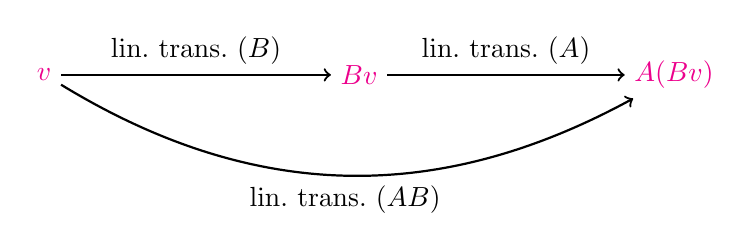
\begin{tikzpicture}
\node[magenta] (v) at (0,0) {\(\vect{v}\)};
\node[magenta] (bv) at (4,0) {\(\vect{Bv}\)};
\node[magenta] (abv) at (8,0) {\(\vect{A(Bv)}\)};
\draw[->, thick] (v) -- (bv)
node[midway,above]{lin.\ trans.\ (\(B\))};
\draw[->, thick] (bv) -- (abv)
node[midway,above]{lin.\ trans.\ (\(A\))};
\draw[->, thick] (v) to[bend right] node[bend right, auto, swap]{lin.\ trans.\ (\(AB\))} (abv);
\end{tikzpicture}
\end{center}
\item \label{it:matrix-mult-explicit}
We can express the matrix product in a more explicit (and more familiar)
form as follows: For any \(i=1,\dotsc,m\) and \(k=1,\dotsc,p\), the
\((i,k)\)-entry of \(AB\) is
\[
(AB)_{\blc{i}\vc{k}}=\sum_{\rc{j}=1}^{n}a_{\blc{i}\rc{j}}b_{\rc{j}\vc{k}}
\]
where we write \(A=[a_{ij}]\) and \(B=[b_{jk}]\). 

Examples:
\begin{itemize}
\item \begin{align*}
\mqty[1&2&3\\ 3&2&1]\mqty[1&0\\ 0&1\\ 1&2]
&=\mqty[
\mqty[\blc{1}&\vc{2}&\orc{3}\\ \blc{3}&\vc{2}&\orc{1}]\mqty[\blc{1}\\ \vc{0}\\ \orc{1}]
&\mqty[\blc{1}&\vc{2}&\orc{3}\\ \blc{3}&\vc{2}&\orc{1}]\mqty[\blc{0}\\ \vc{1}\\ \orc{2}]
]\\
&=\mqty[
\blc{1}\mqty[\blc{1}\\ \blc{3}]+\vc{0}\mqty[\vc{2}\\ \vc{2}]+\orc{1}\mqty[\orc{3}\\ \orc{1}]
&\blc{0}\mqty[\blc{1}\\ \blc{3}]+\vc{1}\mqty[\vc{2}\\ \vc{2}]+\orc{2}\mqty[\orc{3}\\ \orc{1}]
]\\
&=\mqty[4&8\\ 4&4]
\end{align*}

\item \begin{align*}
\mqty[1&2&3\\ \rc{3}&\rc{2}&\rc{1}]\mqty[\rc{1}&0\\ \rc{0}&1\\ \rc{1}&2]
&=\mqty[
\mqty[1&2&3\\ \rc{3}&\rc{2}&\rc{1}]\mqty[\rc{1}\\ \rc{0}\\ \rc{1}]
&\mqty[1&2&3\\ 3&2&1]\mqty[0\\ 1\\ 2]
]\\
&=\mqty[
\rc{1}\mqty[1\\ \rc{3}]+\rc{0}\mqty[2\\ \rc{2}]+\rc{1}\mqty[3\\ \rc{1}]
&0\mqty[1\\ 3]+1\mqty[2\\ 2]+2\mqty[3\\ 1]
]\\
&=\mqty[4&8\\ \rc{4}&4]
\end{align*}
\end{itemize}
\item We can also express the \((i,k)\)-entry of \(AB\) as
\[
(AB)_{\blc{i}\vc{k}}=\vect{a}_{\blc{i}}'\vect{b}_{\vc{k}}
=\mqty[a_{\blc{i}1}&\cdots&a_{\blc{i}n}]
\mqty[b_{1\vc{k}}\\\vdots\\b_{n\vc{k}}]
=\sum_{\rc{j}=1}^{n}a_{\blc{i}\rc{j}}b_{\rc{j}\vc{k}}
\]
where \(\vect{a}_{i}'\) and \(\vect{b}_{k}\) are \(i\)th row of \(A\) and
\(k\)th column of \(B\) respectively. \begin{note}
This is sometimes known as the \defn{dot product} of \(\vect{a}_{i}\) and
\(\vect{b}_{k}\) (which sums the products of the corresponding pairs of entries
in the vectors).
\end{note}

\item We have defined matrix product using a ``by column'' approach. But
actually we can also define it using a ``by row'' approach. First, we write
\[
A=\mqty[\vect{a}_{1}'\\ \vdots\\ \vect{a}_{m}'].
\]
Then, we have
\[
AB=\mqty[\vect{a}_{1}'B\\ \vdots\\ \vect{a}_{m}'B]
\]
where the ``left matrix-vector product'' \(\vect{v}'B\) is defined by
\[
\vect{v}'B=v_1\vect{b}_{1}'+\dotsb+v_n\vect{b}_{n}'
\]
with \(\vect{v}'=\mqty[v_1&\cdots&v_n]\) and \(\displaystyle
B=\mqty[\vect{b}_{1}'\\ \vdots\\ \vect{b}_{n}']\) (so that
\((\vect{v}'B)^{T}=B^T(\vect{v}')^T\) where RHS is consistent with the usual
matrix-vector product).

Examples:
\begin{itemize}
\item \begin{align*}
\mqty[1&2&3\\ 3&2&1]\mqty[1&0\\ 0&1\\ 1&2]
&=\mqty[
\mqty[\blc{1}&\vc{2}&\orc{3}]
\mqty[\blc{1}&\blc{0}\\ \vc{0}&\vc{1}\\ \orc{1}&\orc{2}]\\
\mqty[\blc{3}&\vc{2}&\orc{1}]
\mqty[\blc{1}&\blc{0}\\ \vc{0}&\vc{1}\\ \orc{1}&\orc{2}]
]\\
&=\mqty[
\blc{1}\mqty[\blc{1}&\blc{0}]
+\vc{2}\mqty[\vc{0}&\vc{1}]
+\orc{3}\mqty[\orc{1}&\orc{2}]
\\
\blc{3}\mqty[\blc{1}&\blc{0}]
+\vc{2}\mqty[\vc{0}&\vc{1}]
+\orc{1}\mqty[\orc{1}&\orc{2}]
]\\
&=\mqty[4&8\\ 4&4]
\end{align*}

\item \begin{align*}
\mqty[1&2&3\\ \rc{3}&\rc{2}&\rc{1}]\mqty[\rc{1}&0\\ \rc{0}&1\\ \rc{1}&2]
&=\mqty[
\mqty[1&2&3]
\mqty[1&0\\ 0&1\\ 1&2]\\
\mqty[\rc{3}&\rc{2}&\rc{1}]
\mqty[\rc{1}&0\\ \rc{0}&1\\ \rc{1}&2]
]\\
&=\mqty[
1\mqty[1&0]
+2\mqty[0&1]
+3\mqty[1&2]
\\
\rc{3}\mqty[\rc{1}&0]
+\rc{2}\mqty[\rc{0}&1]
+\rc{1}\mqty[\rc{1}&2]
]\\
&=\mqty[4&8\\ \rc{4}&4]
\end{align*}
\end{itemize}
\item Another remarkable approach for matrix multiplication is \emph{block
multiplication}, which can be helpful especially when the sizes of the matrices
involved are large.

The basic idea of \defn{block multiplication} is to divide a large matrix into
several partitions or \emph{blocks}, and ``treat'' each block like a scalar.
Then, it turns out that performing matrix multiplication as usual under this
treatment results in a correct matrix product (which can be proved
mathematically).

\item From a ``partition'' perspective, the previous ``by column'' (``by row'')
definition of matrix multiplication is actually indeed just block
multiplication with the matrix \(B\) (\(A\)) having columns (rows)
partitioned, and the whole matrix \(A\) (\(B\)) treated as a single block (a
matrix with one ``block entry'') respectively.
\begin{itemize}
\item (``by column'') \[
AB=\mqty[A]\mqty[\vect{b}_{1}&\cdots&\vect{b}_{p}]
\overset{\text{entries treated as scalars}}{=}\mqty[A\vect{b}_{1}&\cdots&A\vect{b}_{p}].
\]
\item (``by row'') \[
AB=\mqty[\vect{a}_{1}'\\ \vdots\\ \vect{a}_{m}']\mqty[B]
\overset{\text{entries treated as scalars}}{=}\mqty[\vect{a}_{1}'B\\ \vdots\\ \vect{a}_{m}'B].
\]
\end{itemize}

\item In general, under block multiplication, we can partition a matrix into
\emph{rectangular blocks}/submatrices (partition \emph{both} rows and columns),
and then carry out the matrix multiplication (treating each block as scalar),
\emph{as long as} matrix multiplication under such treatment is
\emph{well-defined}.

To ensure the well-definedness, for matrix product \(AB\), the \emph{columns}
of \(A\) and the \emph{rows} of \(B\) should be partitioned in the \emph{same
pattern}. Example:
\[
\mqty[
\blc{1}&\blc{2}&\blc{1}&\vc{3}&\vc{5}\\
\blc{0}&\blc{7}&\blc{0}&\vc{3}&\vc{1}\\
\blc{1}&\blc{5}&\blc{1}&\vc{4}&\vc{3}\\
]
\mqty[
\rc{2}&\rc{5}\\
\rc{1}&\rc{6}\\
\rc{0}&\rc{0}\\
\gc{1}&\gc{1}\\
\gc{2}&\gc{1}
]
=
\mqty[
\blc{1}&\blc{2}&\blc{1}\\
\blc{0}&\blc{7}&\blc{0}\\
\blc{1}&\blc{5}&\blc{1}\\]
\mqty[
\rc{2}&\rc{5}\\
\rc{1}&\rc{6}\\
\rc{0}&\rc{0}\\]
+\mqty[
\vc{3}&\vc{5}\\
\vc{3}&\vc{1}\\
\vc{4}&\vc{3}\\]
\mqty[\gc{1}&\gc{1}\\
\gc{2}&\gc{1}\\].
\]
\item To justify the block multiplication approach, we can utilize the explicit
form of matrix multiplication in \labelcref{it:matrix-mult-explicit}.
Intuitively, each ``partition'' in block multiplication indeed corresponds to
a certain ``splitting'' of the sum. For example, in the block multiplication
\[
\mqty[
\blc{1}&\blc{2}&\blc{1}&\vc{3}&\vc{5}\\
\blc{0}&\blc{7}&\blc{0}&\vc{3}&\vc{1}\\
\blc{1}&\blc{5}&\blc{1}&\vc{4}&\vc{3}\\
]
\mqty[
\rc{2}&\rc{5}\\
\rc{1}&\rc{6}\\
\rc{0}&\rc{0}\\
\gc{1}&\gc{1}\\
\gc{2}&\gc{1}
]
=
\mqty[
\blc{1}&\blc{2}&\blc{1}\\
\blc{0}&\blc{7}&\blc{0}\\
\blc{1}&\blc{5}&\blc{1}\\]
\mqty[
\rc{2}&\rc{5}\\
\rc{1}&\rc{6}\\
\rc{0}&\rc{0}\\]
+\mqty[
\vc{3}&\vc{5}\\
\vc{3}&\vc{1}\\
\vc{4}&\vc{3}\\]
\mqty[\gc{1}&\gc{1}\\
\gc{2}&\gc{1}\\],
\]
the \((1,1)\)-entry can be obtained by
\[
\blc{1}\cdot\rc{2}+\blc{2}\cdot\rc{1}+\blc{1}\cdot\rc{0}
+\vc{3}\cdot \gc{1}+\vc{5}\cdot \gc{2}
\overset{\text{split}}{=}(\blc{1}\cdot\rc{2}+\blc{2}\cdot\rc{1}+\blc{1}\cdot\rc{0})
+(\vc{3}\cdot \gc{1}+\vc{5}\cdot \gc{2}).
\]

\item To close \cref{subsect:matrix-mult}, we introduce the concept of
\emph{matrix power}.  If \(A\) is a \emph{square} matrix and \(k\) is a
positive integer, then the \defn{\(k\)th power of \(A\)} is
\[
A^k=\underbrace{AA\cdots A}_{\text{\(k\) times}}.
\]
\end{enumerate}
\subsection{Properties of Matrix Multiplication}
\label{subsect:matrix-mult-prop}
\begin{enumerate}
\item Here we will introduce several properties of matrix multiplication. To
prove them, we will mainly utilize the explicit form of matrix
multiplication in \labelcref{it:matrix-mult-explicit}.

\item \label{it:matrix-mult-asso}
The first property is \emph{associativity} (like matrix addition). Let
\(A\), \(B\), and \(C\) be \(m\times n\), \(n\times p\), and \(p\times q\)
matrices respectively. Then, we have
\[
(AB)C=A(BC).
\]
\begin{pf}
For any \(i=1,\dotsc,m\) and \(\ell=1,\dotsc,q\),
\begin{align*}
[(AB)C]_{i\ell }&=\sum_{k=1}^{p}\vc{(AB)_{ik}}C_{k\ell}\\
&=\sum_{k=1}^{p}\vc{\sum_{j=1}^{n}A_{ij}B_{jk}}C_{k\ell}\\
&=\sum_{j=1}^{n}\sum_{k=1}^{p}A_{ij}B_{jk}C_{k\ell}&\text{(switching summation order)}\\
&=\sum_{j=1}^{n}\underbrace{A_{ij}}_{\text{independent of \(k\)}}\gc{\sum_{k=1}^{p}B_{jk}C_{k\ell}}\\
&=\sum_{j=1}^{n}A_{ij}\gc{(BC)_{j\ell}}\\
&=[A(BC)]_{i\ell}.
\end{align*}
\end{pf}

\item \label{it:matrix-mult-dist}
The next one is \emph{distributivity} (like matrix addition again). Let \(A\)
be an \(m\times n\) matrix, and let \(B\) and \(C\) be \(n\times p\) matrices.
Then,
\[
A(B+C)=AB+AC.
\]
\begin{pf}
For any \(i=1,\dotsc,m\) and \(k=1,\dotsc,p\),
\begin{align*}
[A(B+C)]_{ik}&=\sum_{j=1}^{n}A_{ij}(B+C)_{jk}\\
&=\sum_{j=1}^{n}A_{ij}(B_{jk}+C_{jk})\\
&=\sum_{j=1}^{n}(A_{ij}B_{jk}+A_{ij}C_{jk})\\
&=\sum_{j=1}^{n}A_{ij}B_{jk}+\sum_{j=1}^{n}A_{ij}C_{jk}\\
&=(AB)_{ik}+(AC)_{ik}.
\end{align*}
\end{pf}

The above property is \emph{left-distributivity} to be more specific. The
\emph{right-distributivity} also holds, but we need to adjust the sizes of the
matrices:
\[
(A+B)C=AC+BC
\]
when \(A\) and \(B\) are \(m\times n\) matrices, and \(C\) is an \(n\times p\)
matrix.

\begin{pf}
Similar to the proof above.
\end{pf}

\item \label{it:matrix-mult-noncomm}
This ``property'' is of particular importance: \emph{\underline{non}-commutativity} (\warn{}
\underline{unlike} matrix addition!). Even for two square matrices \(A\) and
\(B\), we do \emph{not} always have
\[
AB=BA!
\]
\begin{pf}
To prove this, it suffices to give a counterexample. Take \(A=\mqty[1&1\\
0&1]\) and \(B=\mqty[1&0\\ 1&1]\). Then,
\[
AB=\mqty[2&1\\ 1&1]\qqtext{while}
BA=\mqty[1&1\\ 1&2].
\]
\end{pf}

\item \label{it:matrix-prod-transpose-anticomm}
The final property we discuss here is related to \emph{matrix transpose}.
Let \(A\) be an \(m\times n\) matrix and \(B\) be an \(n\times p\). Then we
have the following \emph{anti-commutativity} for transpose of \(AB\):
\[
(AB)^{T}=B^{T}A^{T}.
\]
\begin{pf}
For any \(i=1,\dotsc,m\) and \(k=1,\dotsc,p\), we have
\begin{align*}
[(AB)^{T}]_{ki}&=(AB)_{ik}\\
&=\sum_{\rc{j}=1}^{n}A_{i\rc{j}}B_{\rc{j}k}\\
&=\sum_{\rc{j}=1}^{n}(B^T)_{k\rc{j}}(A^T)_{\rc{j}i}\\
&=(B^{T}A^{T})_{ki}.
\end{align*}
\end{pf}
\end{enumerate}
\subsection{Determinants}
\begin{enumerate}
\item \label{it:deter-geo}
Recall the ``linear transformation'' interpretation of a square matrix in
\labelcref{it:sq-matrix-geo-interpret}. Basically, the concept of
\emph{determinant} aims to ``quantify'' the linear transformation
``represented'' by the square matrix. 

More specifically, the \emph{determinant} of an \(n\times n\) square matrix is
the \emph{signed} ``area''\footnote{For the \(2\times 2\) case, this means that
the area ``above'' (``below'') the vector linearly transformed from
\(\vect{i}\) contributes positively (negatively) to this quantity, and the area
on the ``right'' (``left'') of the vector linearly transformed from \(\vect{j}\)
contributes positively (negatively) to this quantity.} (or its analogue in
other dimension) of the geometrical object ``spanned'' by the vectors linearly
transformed from the standard vectors (loosely, ``parallelogram'' (or its
analogue in other dimension, e.g., parallelepiped in 3-dimensional case) with
those transformed vectors as sides).

\begin{center}
\begin{tikzpicture}
\draw[-Latex] (-3,0) -- (3,0);
\draw[-Latex] (0,-3) -- (0,3);
\draw[->, very thick, blue, opacity=0.5] (0,0) -- (1,0);
\node[blue, opacity=0.5] () at (1.2,-0.3) {\(\vect{i}\)};
\draw[->, very thick, violet, opacity=0.5] (0,0) -- (0,1);
\node[violet, opacity=0.5] () at (-0.3,1.2) {\(\vect{j}\)};
\draw[->, blue, very thick] (0,0) -- (0.5,0.866)
node[pos=1.6, font=\small]{\(\mqty[0.5\\ \sqrt{3}/2]\)};
\draw[->, violet, very thick] (0,0) -- (-0.866,0.5)
node[pos=1.6, font=\small]{\(\mqty[-\sqrt{3}/2\\ 0.5]\)};
\node[] () at (0,-3.5) {\(A=\mqty[\cos\pi/3&-\sin\pi/3\\ \sin\pi/3&\cos\pi/3]=\mqty[0.5&-\sqrt{3}/2\\ \sqrt{3}/2&0.5]\)};
\draw[rotate=60, fill=green!30!white, draw=none, opacity=0.3] (0,0) rectangle (1,1);
\end{tikzpicture}
\begin{tikzpicture}
\draw[-Latex] (-3,0) -- (3,0);
\draw[-Latex] (0,-3) -- (0,3);
\draw[->, very thick, blue, opacity=0.5] (0,0) -- (1,0);
\node[blue, opacity=0.5] () at (1.2,-0.3) {\(\vect{i}\)};
\draw[->, very thick, violet, opacity=0.5] (0,0) -- (0,1);
\node[violet, opacity=0.5] () at (-0.3,1.2) {\(\vect{j}\)};
\draw[->, blue, thick] (0,0) -- (2,0);
\node[blue] () at (2,-0.7) {\(\mqty[2\\ 0]\)};
\draw[->, violet, thick] (0,0) -- (0,2);
\node[violet] () at (0.5,1.5) {\(\mqty[0\\ 2]\)};
\node[] () at (0,-3.5) {\(B=\mqty[2&0\\ 0&2]\)};
\draw[fill=green!30!white, draw=none, opacity=0.3] (0,0) rectangle (2,2);
\end{tikzpicture}
\begin{tikzpicture}
\draw[-Latex] (-1,0) -- (6,0);
\draw[-Latex] (0,-1) -- (0,4);
\draw[->, very thick, blue, opacity=0.5] (0,0) -- (1,0);
\node[blue, opacity=0.5] () at (1.2,-0.3) {\(\vect{i}\)};
\draw[->, very thick, violet, opacity=0.5] (0,0) -- (0,1);
\node[violet, opacity=0.5] () at (-0.3,1.2) {\(\vect{j}\)};
\draw[->, blue, thick] (0,0) -- (1.5,0);
\node[blue] () at (1.8,-0.7) {\(\mqty[1.5\\ 0]\)};
\draw[->, violet, thick] (0,0) -- (2,1);
\node[violet] () at (2,1.5) {\(\mqty[2\\ 1]\)};
\draw[fill=green!30!white, draw=none, opacity=0.3, xslant=2] (0,0) rectangle (1.5,1);
\node[] () at (3,3) {\(C=\mqty[1.5&2\\ 0&1]\)};
\end{tikzpicture}
\end{center}
\item First, we consider a special case where \(n=1\). In such case, instead of
considering signed \emph{area}, we consider a \emph{lower-dimensional}
analogue: signed \emph{length}. In the \(n=1\) case, the \defn{determinant of a
\(1\times 1\) matrix} (which is just a scalar essentially) \([a]\) is just
the signed length of line segment joining \(0\) and \(a\) in the real number
line, namely \(\boxed{a}\).
\begin{center}
\begin{tikzpicture}
\draw[-Latex] (-5,0) -- (5,0);
\draw[fill, blue] (3,0) circle [radius=0.5mm];
\draw[fill, blue] (0,0) circle [radius=0.5mm];
\node[] () at (3,0.3) {\(3\)};
\draw[fill, blue] (-4,0) circle [radius=0.5mm];
\node[] () at (-4,0.3) {\(-4\)};
\node[] () at (0,0.3) {\(0\)};
\draw[magenta] (0,0) -- (3,0)
node[midway, below]{signed length: \(3\)};
\draw[brown] (-4,0) -- (0,0)
node[midway, below]{signed length: \(-4\)};
\end{tikzpicture}
\end{center}
\begin{note}
The determinant of a matrix \(A\) is denoted by \(\det A\) or \(|A|\).
When, we
write out the entries of \(A\) explicitly like \(A=\mqty[a&b\\ c&d]\), we can
also denote its determinant by \(\mqty|a&b\\ c&d|\) (replacing the brackets by
vertical bars).
\begin{warning}
It may lead to some ambiguity for the \(1\times 1\) matrix case as we would
just write \(|a|\), which may be understood as the absolute value of \(a\)
(\underline{not} the determinant of \(1\times 1\) matrix \([a]\)!).
\end{warning}
\end{note}
\item For \(2\times 2\) and \(3\times 3\) matrices, the determinant is defined
as follows (which turns out to coincide with the geometrical interpretation in
\labelcref{it:deter-geo}, by considering \emph{cross product} (\(2\times 2\)
case) and \emph{scalar triple product} (\(3\times 3\) case)):
\begin{itemize}
\item The \defn{determinant of a \(2\times 2\) matrix} \(\mqty[a&b\\ c&d]\) is
\[
\boxed{\gc{ad}\rc{-bc}}.
\]
\item The \defn{determinant of a \(3\times 3\) matrix} \(\mqty[a&b&c\\ d&e&f\\ g&h&i]\) is
\[
\boxed{\gc{aei}\blc{+bfg}\vc{+cdh}\rc{-ceg}\mgc{-bdi}\orc{-afh}}.
\]
\end{itemize}
\begin{mnemonic}
Both expressions can be viewed via ``diagonal multiplication'':
\begin{center}
\begin{tikzpicture}
\node[] () at (0,0) {\(\mqty[a&b\\ c&d]\)};
\draw[-Latex, green!50!black] (-0.5,0.5) -- (0.5,-0.5)
node[pos=1.2]{\(+ad\)};
\draw[-Latex, red] (0.5,0.5) -- (-0.5,-0.5)
node[pos=1.2]{\(-bc\)};
\end{tikzpicture}
\end{center}
\begin{center}
\begin{tikzpicture}
\node[] () at (0,0) {\(\mqty[a&b&c\\ d&e&f\\ g&h&i]\)};
\draw[-Latex, green!50!black] (-1,0.8) -- (1,-0.8)
node[pos=1.1]{\(+aei\)};
\draw[-Latex, blue] (-0.4,0.8) -- (0.9,-0.3);
\draw[-Latex, blue] (-1,0) -- (-0.2,-0.8)
node[pos=1.2]{\(+bfg\)};
\draw[-Latex, violet] (-1,0.4) -- (0.4,-0.8);
\draw[-Latex, violet] (0.2,0.8) -- (1,0)
node[pos=1.2]{\(+cdh\)};
\end{tikzpicture}
\begin{tikzpicture}
\node[] () at (0,0) {\(\mqty[a&b&c\\ d&e&f\\ g&h&i]\)};
\draw[-Latex, red] (1,0.8) -- (-1,-0.8)
node[pos=1.1]{\(-ceg\)};
\draw[-Latex, magenta] (0.4,0.8) -- (-0.9,-0.3);
\draw[-Latex, magenta] (1,0) -- (0.2,-0.8)
node[pos=1.2]{\(-bdi\)};
\draw[-Latex, orange!90!black] (1,0.4) -- (-0.4,-0.8);
\draw[-Latex, orange!90!black] (-0.2,0.8) -- (-1,0)
node[pos=1.3]{\(-afh\)};
\end{tikzpicture}
\end{center}
\end{mnemonic}


\item Observe that the determinant of a \(3\times 3\) matrix can actually be
expressed in terms of determinants of \(2\times 2\) matrices:
\begin{align*}
\mqty|a&b&c\\ d&e&f\\ g&h&i|
&=aei+bfg+cdh-ceg-bdi-afh\\
&=a(ei-fh)-b(di-fg)+c(dh-eg)\\
&=a\mqty|e&f\\ h&i|-b\mqty|d&f\\ g&i|+c\mqty|d&e\\ g&h|.
\end{align*}
Indeed, the determinant of a \(2\times 2\) matrix can also be expressed in
terms of determinants of \(1\times 1\) ``matrices'' (which are scalars
essentially), obviously:
\[
\mqty|a&b\\ c&d|
=ad-bc
=a\det[d]-b\det[c].
\]

Additionally, we have the following observations:
\begin{itemize}
\item The signs of the terms are alternating (``chessboard pattern'': \(+\),
\(-\), \(+\), ...).
\item The coefficients of the determinants are taken from the first row of the
original matrix (without considering sign).
\item The ``smaller'' determinants are determinants of some submatrices of the
original. In fact, they are obtained by deleting a row and a column:
\begin{center}
\begin{tikzpicture}
\node[] (33det) at (0,0) {\(\mqty|\blc{a}&b&c\\ d&e&f\\ g&h&i|\)};
\draw[red] (-1,0.45) -- (1,0.45);
\draw[red] (-0.55,0.7) -- (-0.55,-0.7);
\node[] (22det) at (3,0) {\(\mqty|e&f\\ h&i|\)};
\draw[-Latex] (33det) -- (22det);
\end{tikzpicture}
\quad
\begin{tikzpicture}
\node[] (33det) at (0,0) {\(\mqty|a&\blc{b}&c\\ d&e&f\\ g&h&i|\)};
\draw[red] (-1,0.45) -- (1,0.45);
\draw[red] (0,0.7) -- (0,-0.7);
\node[] (22det) at (3,0) {\(\mqty|d&f\\ g&i|\)};
\draw[-Latex] (33det) -- (22det);
\end{tikzpicture}
\quad
\begin{tikzpicture}
\node[] (33det) at (0,0) {\(\mqty|a&b&\blc{c}\\ d&e&f\\ g&h&i|\)};
\draw[red] (-1,0.45) -- (1,0.45);
\draw[red] (0.55,0.7) -- (0.55,-0.7);
\node[] (22det) at (3,0) {\(\mqty|d&e\\ g&h|\)};
\draw[-Latex] (33det) -- (22det);
\end{tikzpicture}
\end{center}
\end{itemize}
These lead to the following general (\emph{cofactor expansion}) definition of
determinant.

\item Let \(A=[a_{ij}]\) be an \(n\times n\) matrix with \(n\ge 2\). Let
\(\widetilde{A}_{ij}\) be the \((n-1)\times (n-1)\) matrix obtained by deleting
the \(i\)th row and the \(j\)th column of \(A\).

Then, we have the following terminologies:
\begin{itemize}
\item The \defn{\((i,j)\)-minor} of \(A\) is \(\det \widetilde{A}_{ij}\).
\item The \defn{\((i,j)\)-cofactor} of \(A\) is \(C_{ij}=(-1)^{i+j}\det \widetilde{A}_{ij}\).
\item The \defn{cofactor matrix} of \(A\) is an \(n\times n\) matrix \([C_{ij}]\).
\end{itemize}

\begin{note}
When \(i+j\) is odd (even), the sign for the \((i,j)\)-cofactor is negative
(positive). The following shows the sign for the cofactor at different
locations (corresponding to different values of \(i\) and \(j\)) for some
cases, which are of ``chessboard pattern'':
\[
\mqty[+&-\\ +&-]\quad
\mqty[+&-&+\\ -&+&-\\ +&-&+]\quad
\mqty[+&-&+&-\\ +&-&+&-\\ +&-&+&-\\ +&-&+&-]
\]
\end{note}

The \defn{determinant} of \(A\) is then (recursively) defined as
\[
\det A=a_{11}C_{11}+a_{12}C_{12}+\dotsb+a_{1n}C_{1n}.
\]
\begin{remark}
\item This process is also known as \emph{cofactor expansion along the first row}.
\item This definition is \emph{recursive} since the definition for \(n\times
n\) determinant utilizes the notion of \((n-1)\times (n-1)\) determinant, which
is assumed to be already defined.
\item Note that this definition does not include the case for \(1\times 1\)
matrix. However, we have already defined that \(\det [a]=a\).
\item It is not hard to verify that the previous definitions of determinants of
\(2\times 2\) and \(3\times 3\) matrices are consistent with this general
definition.
\end{remark}

\item The general definition of determinant allows us to compute the
determinant of a matrix with size larger than \(3\times 3\). Examples:
\begin{itemize}
\item 
\(\displaystyle 
\mqty|2&0&0&3\\ 1&2&0&-1\\ -2&1&2&0\\ 0&-3&1&2|
=2\mqty|2&0&-1\\ 1&2&0\\ -3&1&2|\rc{-}3\mqty|1&2&0\\ -2&1&2\\ 0&-3&1|
=2(1)-3(11)=-31.
\)
\item \(\det I_n=1\) for any \(n\in\N\).

\begin{pf}
Firstly, we have \(\det I_1=1\). Then, assume for induction that \(\det I_k=1\)
for a certain \(k\in\N\). Then,
\[
\det I_{k+1}=1\cdot \det I_k+\underbrace{0+\dotsb+0}_{\text{\(k-1\) times}}
=\det I_k=1.
\]
Thus, the result follows by induction.
\end{pf}
\end{itemize}
\begin{warning}
The ``diagonal multiplication'' does \underline{not} hold for (square) matrices
with size larger than \(3\times  3\). A counterexample is
\[
\mqty[0&1&0&0\\ 1&0&0&0\\ 0&0&1&0\\ 0&0&0&1]
\]
where the ``diagonal multiplication'' yields \(0\), but the actual determinant
(found by cofactor expansion along the first row) is \(-1\).
\end{warning}
\item The \emph{definition} of determinant utilizes cofactor expansion along
the \emph{first row}. Naturally, one may then ask whether we can perform
cofactor expansion along other row (or even column) or not. It turns out
cofactor expansion along \emph{any} row or column gives the same result, by the
\emph{cofactor expansion theorem}.

\begin{theorem}[Cofactor expansion theorem]
\label{thm:cofactor-expansion}
Let \(A=[a_{ij}]\) be an \(n\times n\) matrix with the \((i,j)\)-cofactor being
\(C_{ij}\). Then, we have
\[
\det A=a_{i1}C_{i1}+\dotsb+a_{in}C_{in}\quad\text{(cofactor expansion along the \(i\)th row)}
\]
for any \(i=1,\dotsc,n\), and
\[
\det A=a_{1j}C_{1j}+\dotsb+a_{nj}C_{nj}\quad\text{(cofactor expansion along the \(j\)th column)}
\]
for any \(j=1,\dotsc,n\).
\end{theorem}
\begin{warning}
Be careful about the signs of the cofactors!
\end{warning}

\item The cofactor expansion theorem is helpful for simplifying (possibly
substantially) the computations of determinants (compared with cofactor
expansion along the first row). Examples:
\begin{itemize}
\item \(\displaystyle 
\mqty|
1&2&3&0&4\\
\rc{1}&\rc{0}&\rc{0}&\rc{0}&\rc{0}\\
4&3&2&2&1\\
-1&-2&0&0&2\\
2&-3&-2&0&-1
|
=\vc{-}\rc{1}\mqty|
2&3&\blc{0}&4\\
3&2&\blc{2}&1\\
-2&0&\blc{0}&2\\
-3&-2&\blc{0}&-1
|+0
=
\blc{2}\mqty|
2&3&4\\
-2&0&2\\
-3&-2&-1
|
=2(0)
=0.
\)
\item The determinant of a triangular (upper triangular or lower triangular)
matrix is the product of all its diagonal entries.

\begin{pf}
WLOG, suppose the matrix is upper triangular (the argument is similar for lower
triangular matrix). Then, it is of the form
\[
\mqty[
a_{11}&a_{12}&\cdots&a_{1,n-1}&a_{1n}\\
0&a_{22}&\cdots&a_{2,n-1}&a_{2n}\\
\vdots&\vdots&\ddots&\vdots&\vdots\\
0&0&\cdots&0&a_{nn}
].
\]
Now performing cofactor expansion along the last (\(n\)th) row gives
\[
\mqty|
a_{11}&a_{12}&\cdots&a_{1,n-1}&a_{1n}\\
0&a_{22}&\cdots&a_{2,n-1}&a_{2n}\\
\vdots&\vdots&\ddots&\vdots&\vdots\\
0&0&\cdots&0&a_{nn}
|
=a_{nn}\mqty|
a_{11}&a_{12}&\cdots&a_{1,n-2}&a_{1,n-1}\\
0&a_{22}&\cdots&a_{2,n-2}&a_{2,n-1}\\
\vdots&\vdots&\ddots&\vdots&\vdots\\
0&0&\cdots&0&a_{n,n-1}
|.
\]
For the matrix on RHS, performing cofactor expansion along the last (\(n-1\)th)
row gives
\[
a_{nn}a_{n-1,n-1}\mqty|
a_{11}&a_{12}&\cdots&a_{1,n-3}&a_{1,n-2}\\
0&a_{22}&\cdots&a_{2,n-3}&a_{2,n-2}\\
\vdots&\vdots&\ddots&\vdots&\vdots\\
0&0&\cdots&0&a_{n,n-2}
|
\]
Repeating this process, we know that the determinant is
\[
a_{nn}a_{n-1,n-1}\dotsb a_{11},
\]
the product of all its diagonal entries.
\end{pf}

\end{itemize}
\item \label{it:deter-block-triang}
It turns out that we have a similar result regarding the determinant of a
\defn{block triangular matrix} (i.e., when viewing the blocks as scalars (zero
matrix \faIcon{arrow-right} zero scalar), the matrix is triangular).

Consider an \(n\times n\) matrix \(A\) which is block triangular, i.e.,
\[
A=\mqty[
A_{11}&*&\cdots&*\\
O&A_{22}&\cdots&*\\
\vdots&\vdots&\ddots&\vdots\\
O&O&\cdots&A_{kk}
]
\qqtext{or}
A=\mqty[
A_{11}&O&\cdots&O\\
*&A_{22}&\cdots&O\\
\vdots&\vdots&\ddots&\vdots\\
*&*&\cdots&A_{kk}
].
\]
\footnote{\(*\)'s denote arbitrary blocks (with appropriate sizes).}
Suppose that \(A_{ii}\) is a square matrix for any \(i=1,\dotsc,n\). Then,
\[
\det A=\det A_{11}\times \dotsb\times \det A_{nn},
\]
i.e., the determinant of \(A\) is the product of the \emph{determinants} of all
its diagonal \emph{blocks}.
\end{enumerate}
\subsection{Properties of Determinants}
\label{subsect:det-prop}
\begin{enumerate}
\item In general, computing determinants can be quite laborious and tedious
(especially for large matrices). So, here we introduce some properties of
determinants that can simplify the computations of determinants (in some
cases).

\item The first property suggests the effect of \emph{switching rows} on the
determinant. It is also known as the \emph{alternating} property (as the sign
``alternates'' through switching rows).
\begin{proposition}[Alternating]
\label{prp:det-alter}
Let \(A=[a_{ij}]\) be an \(n\times  n\) matrix. Suppose that \(B=[b_{ij}]\) is obtained from
\(A\) by switching two of its rows. Then,
\[
\det B=-\det A.
\]
\end{proposition}
\begin{pf}
WLOG, we can assume that the two rows being switched are adjacent. (For
switching of two non-adjacent rows, we can show that it is equivalent to
switching adjacent rows for \emph{odd number} of times \faIcon{arrow-right}
\((-1)^{\text{odd number}}=-1\).)

Now, let the two rows being switched be rows \(i\) and \(i+1\). Then, we can
see that for any \(j=1,\dotsc,n\),
\[
\widetilde{A}_{ij}=\widetilde{B}_{i+1,j}
\qqtext{and}
a_{ij}=b_{i+1,j}.
\]
Now, we perform cofactor expansion along the \(i\)th (\(i+1\)th) row for matrix
\(A\) (\(B\)):
\begin{itemize}
\item \(\displaystyle 
\det A
=\sum_{j=1}^{n}a_{\gc{i}j}(-1)^{\gc{i}+j}\det \widetilde{A}_{\gc{i}j}.
\)
\item \(\displaystyle 
\det B
=\sum_{j=1}^{n}b_{\gc{i+1},j}(-1)^{\gc{i+1}+j}\det \widetilde{B}_{\gc{i+1},j}
=-\sum_{j=1}^{n}b_{\gc{i+1},j}(-1)^{i+j}\det \widetilde{B}_{\gc{i+1},j}.
\)
\end{itemize}
By comparing the two expressions, we can observe that
\[
\det B=-\det A.
\]
\end{pf}

Example:
\[
\mqty|2&1\\3&-1|
=-\mqty|3&-1\\2&1|.
\]
\item A corollary from \cref{prp:det-alter} is the following.
\begin{corollary}
\label{cor:two-identical-rows-zero-det}
Let \(A\) be an \(n\times  n\) matrix. If \(A\) has two identical rows, then
\(\det A=0\).
\end{corollary}
\begin{pf}
Switching the two identical rows of \(A\) results in the same matrix \(A\). But
then by \cref{prp:det-alter}, we must have
\[
\det A=-\det A\implies 2\det A=0\implies \det A=0.
\]
\end{pf}

Example:
\[
\mqty|\gc{1}&\gc{2}&\gc{3}&\gc{4}&\gc{5}\\ 0&1&3&3&1\\ 2&1&0&1&2\\ \gc{1}&\gc{2}&\gc{3}&\gc{4}&\gc{5}\\ 1&1&7&5&9|
=0.
\]

\item The next property is about \emph{adding a scalar multiple of row vector
to a row}. It is also known as \emph{multilinearity} since it suggests a
``linearity'' property on each row (when there are multiple rows in a matrix).
\begin{proposition}[Multilinearity]
\label{prp:det-multilinear}
Let \(\vect{r}_{1},\dotsc,\vect{r}_{n}\) be \(1\times n\) row vectors and let
\(\vect{u}\) be another \(1\times n\) row vector. Let \(c\in\R\). Then,
\[
\det\mqty[\vect{r}_{1}\\\vdots\\ \vect{r}_{i-1}\\ \vect{r}_{i}+\rc{c}\blc{\vect{u}}\\
\vect{r}_{i+1}\\ \vdots\\ \vect{r}_{n}]
=
\det\mqty[\vect{r}_{1}\\\vdots\\ \vect{r}_{i-1}\\ \vect{r}_{i}\\
\vect{r}_{i+1}\\ \vdots\\ \vect{r}_{n}]
+\rc{c}\det\mqty[\vect{r}_{1}\\\vdots\\ \vect{r}_{i-1}\\ \blc{\vect{u}}\\
\vect{r}_{i+1}\\ \vdots\\ \vect{r}_{n}]
\]
\end{proposition}
\begin{pf}
For convenience, we denote the equality above by
\[
\det A=\det B+c\det C.
\]
We then perform cofactor expansion along the \(i\)th row for evaluating \(\det
A\), \(\det B\), and \(\det C\). First, note that for any \(j=1,\dotsc,n\),
\[
\widetilde{A}_{ij}=\widetilde{B}_{ij}=\widetilde{C}_{ij}.
\]
We denote the common \emph{\((i,j)\)-cofactor} by \(C_{ij}\) (without
\(\widetilde{\;}\)).

Now, write \(\vect{r}_{i}=\mqty[r_{i1}&\cdots&r_{in}]\) and
\(\vect{u}=\mqty[u_1&\cdots&u_n]\). Then, we have:
\begin{itemize}
\item \(\displaystyle \det A=\sum_{j=1}^{n}(r_{ij}+cu_{j})C_{ij}=\sum_{j=1}^{n}r_{ij}C_{ij}+c\sum_{j=1}^{n}u_{j}C_{ij}.\)
\item \(\displaystyle \det B=\sum_{j=1}^{n}r_{ij}C_{ij}.\)
\item \(\displaystyle \det C=\sum_{j=1}^{n}u_{j}C_{ij}.\)
\end{itemize}
It is then not hard to see that the equality holds.
\end{pf}

Example:
\[
\mqty|1&1&1\\ 2&3&4\\ 3&4&5|
=\mqty|1&1&1\\ 2&3&4\\ 3&4&5|+\underbrace{\mqty|1&1&1\\ \blc{1}&\blc{1}&\blc{1}\\ 3&4&5|}_{0}
=\mqty|1&1&1\\ 3&4&5\\ 3&4&5|
=0.
\]
\item The next property is about matrix transpose. It turns out that taking
transpose does not affect the determinant.
\begin{proposition}
\label{prp:trans-not-affect-det}
Let \(A=[a_{ij}]\) be an \(n\times n\) matrix (where \(n\in\N\)). Then, \(\det
A^{T}=\det A\).
\end{proposition}
\begin{pf}
We prove this by induction. The case \(n=1\) clearly holds since the transpose
of a \(1\times 1\) matrix is still the \(1\times 1\) matrix itself. Next,
assume that the result holds for \(n=k\), for a certain \(k\in\N\). Now,
consider the case \(n=k+1\) (where \(A\) is a \((k+1)\times (k+1)\) matrix).

Firstly, performing cofactor expansion along the first row for \(\det A\) gives
\[
\det A=\sum_{j=1}^{k+1}a_{1j}(-1)^{1+j}\det\widetilde{A}_{1j}.
\]
Now, write \(A^{T}=[b_{ij}]\) (then \(b_{ij}=a_{ji}\)). Note that for any \(j=1,\dotsc,k+1\),
\((\widetilde{A^{T}})_{j1}=(\widetilde{A}_{1j})^{T}\). Then, by induction
hypothesis we have for any \(j=1,\dotsc,k+1\),
\[
\det (\widetilde{A^{T}})_{j1}
=\det (\widetilde{A}_{1j})^{T}
\overset{\text{induction hypothesis}}{=}\det \widetilde{A}_{1j}
\]
(as \(\widetilde{A}_{1j}\) is of size \(k\times k\)).

Thus, performing cofactor expansion along the first \emph{column} for \(\det
A^{T}\) gives
\[
\det A^{T}
=\sum_{j=1}^{k+1}b_{j1}(-1)^{j+1}\det (\widetilde{A^{T}})_{j1}
=\sum_{j=1}^{k+1}a_{1j}(-1)^{1+j}\det \widetilde{A}_{1j}
=\det A,
\]
so the case \(n=k+1\) holds. Hence, the result follows by induction.
\end{pf}

\item Since taking \emph{transpose} interchanges rows and columns (while
preserving the relative order), \cref{prp:trans-not-affect-det} ``translates''
the previous \emph{alternating} and \emph{multilinear} properties for rows
into the corresponding ``column version'':
\begin{proposition}[Column version of alternating and multilinear properties]
\label{prp:det-alter-multilinear-col-version}
Let \(A\) be an \(n\times n\) matrix. Then,
\begin{enumerate}
\item \label{it:det-alter-col}If two \emph{columns} of \(A\) are switched to obtain a matrix \(B\), then \(\det B=-\det A\).
\item \label{it:two-identical-cols-zero-det}If \(A\) has two identical \emph{columns}, then \(\det A=0\).
\item\label{it:det-multilinear-col} Let \(\vect{c}_{1},\dotsc,\vect{c}_{n}\) be \(n\times 1\) \emph{column}
vectors, and let \(\vect{u}\) be another \(n\times 1\) \emph{column} vector.
Let \(c\in\R\). Then,
\begin{align*}
&\det\mqty[\vect{c}_{1}&\cdots& \vect{c}_{i-1}& \vect{c}_{i}+\rc{c}\blc{\vect{u}}&
\vect{c}_{i+1}& \cdots& \vect{c}_{n}]\\
&\quad=
\det\mqty[\vect{c}_{1}&\cdots& \vect{c}_{i-1}& \vect{c}_{i}&
\vect{c}_{i+1}& \cdots& \vect{c}_{n}]
+\rc{c}\det\mqty[\vect{c}_{1}&\cdots& \vect{c}_{i-1}& \blc{\vect{u}}&
\vect{c}_{i+1}& \cdots& \vect{c}_{n}].
\end{align*}
\end{enumerate}
\end{proposition}
\begin{pf}
They follow from taking transpose on the matrices for the respective results
proved before.
\end{pf}

\begin{intuition}
We can gain some intuition on
\labelcref{it:det-alter-col,it:two-identical-cols-zero-det} by considering the
geometrical interpretation of determinant:
\begin{center}
\begin{tikzpicture}
\draw[-Latex] (-1,0) -- (6,0);
\draw[-Latex] (0,-1) -- (0,4);
\draw[->, very thick, blue, opacity=0.5] (0,0) -- (1,0);
\node[blue, opacity=0.5] () at (1.2,-0.3) {\(\vect{i}\)};
\draw[->, very thick, violet, opacity=0.5] (0,0) -- (0,1);
\node[violet, opacity=0.5] () at (-0.3,1.2) {\(\vect{j}\)};
\draw[->, violet, thick] (0,0) -- (1.5,0);
\node[violet] () at (1.8,-0.7) {\(\mqty[1.5\\ 0]\)};
\draw[->, blue, thick] (0,0) -- (2,1);
\node[blue] () at (2,1.5) {\(\mqty[2\\ 1]\)};
\draw[fill=red!30!white, draw=none, opacity=0.3, xslant=2] (0,0) rectangle (1.5,1);
\node[] () at (3,3) {\(A=\mqty[2&1.5\\ 1&0]\)};
\draw[-Latex] (3.5,1.5) -- (2.2,0.7)
node[pos=-0.5]{negative signed area};
\end{tikzpicture}
\begin{tikzpicture}
\draw[-Latex] (-1,0) -- (6,0);
\draw[-Latex] (0,-1) -- (0,4);
\draw[->, very thick, blue, opacity=0.5] (0,0) -- (1,0);
\node[blue, opacity=0.5] () at (1.2,-0.3) {\(\vect{i}\)};
\draw[->, very thick, violet, opacity=0.5] (0,0) -- (0,1);
\node[violet, opacity=0.5] () at (-0.3,1.2) {\(\vect{j}\)};
\draw[->, blue, very thick] (0,0) -- (2,1);
\node[blue] () at (2,0.3) {\(\mqty[2\\ 1]\)};
\draw[->, violet, thick] (0,0) -- (2,1);
\node[violet] () at (2,1.5) {\(\mqty[2\\ 1]\)};
\draw[fill=green!30!white, draw=none, xslant=2] (0,0) rectangle (0.05,1);
\node[] () at (3,3) {\(A=\mqty[2&2\\ 1&1]\)};
\draw[-Latex] (3,1) -- (2.2,1)
node[pos=-1.3]{zero area};
\end{tikzpicture}
\end{center}
\end{intuition}

\item Next, we consider some properties that apply to the ``whole'' matrix (not
rows or columns). The first one is about scalar multiplication.
\begin{proposition}
\label{prp:det-scalar-mult}
Let \(A\) be an \(n\times n\) matrix and let \(k\in\R\). Then,
\[
\det(kA)=k^n\det A.
\]
\begin{warning}
We do \underline{not} have \(\det(kA)=k\det A\) (unless \(n=1\))!
\end{warning}
\end{proposition}
\begin{pf}
Write \(A=\mqty[\vect{c}_{1}&\vect{c}_{2}&\cdots&\vect{c}_{n}]\). Then,
\[
kA=\mqty[k\vect{c}_{1}&\vect{c}_{2}&\cdots&k\vect{c}_{n}].
\]
Now, applying \labelcref{it:det-multilinear-col} \(n\) times gives
\begin{align*}
\det(kA)&=\det\mqty[k\vect{c}_{1}&k\vect{c}_{2}&\cdots&k\vect{c}_{n}]\\
&=k\det\mqty[\vect{c}_{1}&k\vect{c}_{2}&\cdots&k\vect{c}_{n}]\\
&=k^{2}\det\mqty[\vect{c}_{1}&\vect{c}_{2}&\cdots&k\vect{c}_{n}]\\
&=\dotsb\\
&=k^n\det\mqty[\vect{c}_{1}&\vect{c}_{2}&\cdots&\vect{c}_{n}]\\
&=k^n\det A.
\end{align*}
\end{pf}

\item Apart from scalar multiplication, we also have a property regarding
\emph{matrix multiplication}. It turns out that there is a
\emph{multiplicative} property.
\begin{proposition}[Multiplicative]
\label{prp:det-multiplicative}
Let \(A\) and \(B\) be two \(n\times n\) matrices. Then,
\[
\det(AB)=\det A\det B.
\]
\end{proposition}
\begin{pf}
Deferred to \cref{sect:sle}.
\end{pf}

\item To close \cref{subsect:det-prop}, we introduce a ``rule'' that simplifies
computation of determinants, based on the properties we derive. Consider an
\(n\times n\) matrix \(A\), written by
\[
A=\mqty[\vect{r}_{1}\\ \vdots\\ \vect{r}_{n}].
\]
The ``rule'' is that \emph{subtracting the \(i\)th row of \(A\) by a scalar
multiple of another row of \(A\) does \underline{not} affect the determinant}.
More specifically, fix a \(i=1,\dotsc,n\), and let \(j=1,\dotsc,n\) with \(j\ne
i\). Let \(c\in\R\). Then,
\begin{align*}
\det\mqty[\vect{r}_{1}\\ \vdots\\ \vect{r}_{i}-c\vect{r}_j\\\vdots\\\vect{r}_{j}\\\vdots\\ \vect{r}_{n}]
&=\det\mqty[\vect{r}_{1}\\ \vdots\\ \vect{r}_{i}\\\vdots\\\vect{r}_{j}\\\vdots\\ \vect{r}_{n}]
-c\det\mqty[\vect{r}_{1}\\ \vdots\\ \vect{r}_{j}\\\vdots\\\vect{r}_{j}\\\vdots\\ \vect{r}_{n}]&\text{(\cref{prp:det-multilinear})}\\
&=\det A-c(0)&\text{(\cref{cor:two-identical-rows-zero-det})}\\
&=\det A.
\end{align*}
For convenience, we denote this subtraction by \(-c\vect{r}_{j}+\vect{r}_{i}\to
\vect{r}_{i}\) (``adding \(-c\) times the \(j\)th row to the \(i\)th row, and
putting the result in the \(i\)th row'').  (This will be helpful in \cref{sect:sle}
later.)

\begin{remark}
\item This ``rule'' is usually used to create many zeros in a column, so that
performing cofactor expansion along that column is simple.
\item This also applies similarly for columns, by utilizing the corresponding
properties for columns.
\end{remark}
Example:
\begin{align*}
\mqty|1&0&1&1\\ 2&1&3&1\\ 3&1&-2&1\\ -1&1&1&2|
&=\mqty|\blc{1}&0&1&1\\ 0&\gc{1}&\gc{1}&\gc{-3}\\ 0&\gc{1}&\gc{-5}&\gc{-2}\\ 0&\gc{1}&\gc{2}&\gc{3}|&\text{(\(-2\vect{r}_1+\vect{r}_2\to\vect{r}_{2}\), \(-3\vect{r}_{1}+\vect{r}_{3}\to\vect{r}_{3}\), and \(\vect{r}_{1}+\vect{r}_{4}\to\vect{r}_{4}\))}\\
&=\blc{1}\mqty|\gc{1}&\gc{1}&\gc{-3}\\ \gc{1}&\gc{-5}&\gc{-2}\\ \gc{1}&\gc{2}&\gc{3}|&\text{(cofactor expansion along the first column)}\\
&=\mqty|\blc{1}&1&-3\\ 0&\gc{-6}&\gc{1}\\ 0&\gc{1}&\gc{6}|&\text{(\(-\vect{r}_{1}+\vect{r}_{2}\to\vect{r}_{2}\) and \(-\vect{r}_{1}+\vect{r}_{3}\to\vect{r}_{3}\))}\\
&=\blc{1}\mqty|\gc{-6}&\gc{1}\\ \gc{1}&\gc{6}|&\text{(cofactor expansion along the first column)}\\
&=-36-1=-37.
\end{align*}
\end{enumerate}
\subsection{Matrix Inverses}
\label{subsect:matrix-inv}
\begin{enumerate}
\item The (multiplicative) \emph{inverse} of a real number \(a\) is a real
number \(b\) such that \(ab=1\), which is denoted by \(a^{-1}\). (However, the
inverse may not exist. For example, \(0\) does not have an inverse.) We have a
similar notion for matrices.

\item An \(n\times n\) matrix \(A\) is \defn{invertible} (or
\defn{non-singular}\footnote{Note that ``invertible'' corresponds to
``\underline{non}-singular'' rather than ``singular''. We have this terminology
since a matrix together with its inverse is like a ``couple'', so if a matrix
\emph{has} inverse, then it is not ``singular''.}) if there exists an \(n\times
n\) matrix \(B\) such that \(AB=BA=I_n\).  The matrix \(B\) is is called the
\defn{inverse} of \(A\), and is denoted by \(A^{-1}\). A matrix with no inverse
is called \defn{non-invertible} (or \defn{singular}).

\begin{remark}
\item We only define invertibility for \emph{square matrices}.

\item Compared with the notion of inverse for real numbers, there is an extra
condition: \(AB=BA\) (which may not hold due to the non-commutativity of matrix
multiplication). But it turns out that if we have either \(AB=I_n\) or
\(BA=I_n\), then another one would automatically hold\footnote{This is asserted
by the \emph{invertible matrix theorem}, which gives a series of statements
equivalent to invertibility.}). So, to prove invertibility we only need to show
one of the equalities.
\end{remark}

\item Like the case for real numbers, the matrix inverse is unique (if exist).
\begin{proposition}
\label{prp:matrix-inv-unique}
Let \(A\) be an \(n\times n\) matrix. Then, the inverse of \(A\), if exists,
must be unique.
\end{proposition}
\begin{pf}
Suppose that \(B\) and \(C\) are inverses of \(A\). Then, by definition we have
\[
AB=BA=AC=CA=I_n.
\]
This implies
\[
B=BI_n=B(AC)=(BA)C=I_nC=C,
\]
establishing the uniqueness.
\end{pf}

\item It turns out that there is a special relationship between
\emph{invertibility} and \emph{determinant}. One main result we would like to
prove in \cref{subsect:matrix-inv} is that a matrix \(A\) is invertible
\emph{if and only if} \(\det A\ne 0\).

\item Proving the ``only if'' direction is not too hard:
\begin{proposition}
\label{prp:det-inv-fmla}
Let \(A\) be an invertible \(n\times n\) matrix. Then, \(\det A\ne 0\).
Furthermore, we have
\[
\det(A^{-1})=\frac{1}{\det A}.
\]
\end{proposition}
\begin{pf}
Since \(A\) is invertible, we have \(AA^{-1}=I_n\). Now, taking determinant gives
\[
\det(AA^{-1})=\det I_n=1
\implies
(\det A)(\det(A^{-1}))=1.
\]
This implies \(\det A\ne 0\) (otherwise the product would be \(0\), rather than
\(1\)).  Hence, by rearranging the equation we have
\[
\det(A^{-1})=\frac{1}{\det A}.
\]
\end{pf}

\item On the other hand, proving the ``if'' direction is much more involved. We
first define a related notion: \emph{adjugate matrix}. Let \(A\) be an
\(n\times n\) matrix. Then, the \defn{adjugate} of \(A\), denoted by \(\adj
A\), is the \emph{transpose} of the cofactor matrix of \(A\): \(C=[C_{ij}]\)
with \(C_{ij}=(-1)^{i+j}\det\widetilde{A}_{ij}\) for any \(i,j=1,\dotsc,n\),
i.e.,
\[
\adj A=[C_{ij}]^{T}.
\]

\item An important result for the adjugate matrix is as follows.
\begin{theorem}
\label{thm:a-adj-det-a}
Let \(A=[a_{ij}]\) be an \(n\times n\) matrix. Then,
\[
A(\adj A)=(\det A)I_n=(\adj A)A.
\]
\end{theorem}
\begin{pf}
We prove only the first equality since the second equality can be proved
similarly (row \faIcon{arrows-alt-h} column, etc.). By definition of matrix
multiplication, the \((i,j)\)-entry of \(A\adj A\) is 
\[
a_{i1}C_{j1}+\dotsb+a_{1n}C_{jn}.
\]
When \(i=j\), this equals \(\det A\) by the cofactor expansion theorem
(\cref{thm:cofactor-expansion}). Now consider the case where \(i\ne j\). Let
\(A'\) be the matrix obtained from \(A\) by replacing its \(j\)th row by its
\(i\)th row, i.e.,
\[
A=\mqty[
a_{11}&\cdots&a_{1n}\\
\vdots&\ddots&\vdots\\
\rc{a_{i1}}&\rc{\cdots}&\rc{a_{in}}\\
\vdots&\ddots&\vdots\\
a_{j1}&\cdots&a_{jn}\\
\vdots&\ddots&\vdots\\
a_{n1}&\cdots&a_{nn}\\
]
\to
A'=\mqty[
a_{11}&\cdots&a_{1n}\\
\vdots&\ddots&\vdots\\
\rc{a_{i1}}&\rc{\cdots}&\rc{a_{in}}\\
\vdots&\ddots&\vdots\\
\rc{a_{i1}}&\rc{\cdots}&\rc{a_{in}}\\
\vdots&\ddots&\vdots\\
a_{n1}&\cdots&a_{nn}\\
].
\]
Since \(A'\) has two identical rows, we have \(\det(A')=0\). On the other hand,
by considering cofactor expansion of \(A'\) along \(j\)th row (which equals the
original \(i\)th row of \(A\), yet positioned at \(j\)th row), we see that the
\((i,j)\)-entry of \(A\adj A\) \(a_{i1}C_{j1}+\dotsb+a_{1n}C_{jn}\) is indeed
\(\det A'\). Thus, we conclude that the \((i,j)\)-entry of \(A\adj A\) is \(0\)
when \(i\ne j\).

Hence, we have \(A\adj A=(\det A)I_n\).
\end{pf}

\item The following corollary shows the ``if'' direction.
\begin{corollary}
\label{cor:nonzero-det-inv}
Let \(A\) be an \(n\times n\) matrix with \(\det A\ne 0\). Then, \(A\) is
invertible and
\[
A^{-1}=\frac{1}{\det A}\adj A.
\]
\end{corollary}
\begin{pf}
By \cref{thm:a-adj-det-a}, we have
\[
A(\adj A)=(\det A)I_n=(\adj A)A.
\]
Since \(\det A\ne 0\), we can rewrite this as
\[
A\qty(\frac{1}{\det A}\adj A)=I_n=\qty(\frac{1}{\det A}\adj A)A.
\]
By definition, this means that \(A\) is invertible and
\[
A^{-1}=\frac{1}{\det A}\adj A.
\]
\end{pf}
\item With \cref{prp:det-inv-fmla} and \cref{cor:nonzero-det-inv}, we can prove
our desired result about matrix invertibility and determinant:
\begin{theorem}
\label{thm:inv-iff-nonzero-det}
An \(n\times n\) matrix \(A\) is invertible if and only if \(\det A\ne 0\).
\end{theorem}
\begin{pf}
It follows from \cref{prp:det-inv-fmla} (``only if'') and
\cref{cor:nonzero-det-inv} (``if'').
\end{pf}
\item Lastly, we introduce some properties regarding matrix inverse.
\begin{proposition}
\label{prp:matrix-inv-prop}
Let \(A\) and \(B\) be invertible \(n\times n\) matrices. Let \(c\ne 0\). Then,
\begin{enumerate}
\item \((AB)^{-1}=B^{-1}A^{-1}\);
\item \((cA)^{-1}=c^{-1}A^{-1}\);
\item \((A^{T})^{-1}=(A^{-1})^{T}\);
\item \((A^{-1})^{-1}=A\).
\end{enumerate}
\end{proposition}
\begin{pf}
\begin{enumerate}
\item Note that
\[
(B^{-1}A^{-1})(AB)=B^{-1}(A^{-1}A)B=B^{-1}I_nB=B^{-1}B=I_n.
\]
\item Note that
\[
(c^{-1}A^{-1})(cA)=c^{-1}cA^{-1}A=(1)I_n=I_n.
\]
\item Note that
\[
(A^{-1})^{T}A^{T}=(AA^{-1})^{T}=I_n.
\]
\item Note that
\[
A(\blc{A^{-1}})=I_n,
\]
so \(A\) serves as the inverse of \(\blc{A^{-1}}\).
\end{enumerate}
\end{pf}
\end{enumerate}
